\documentclass[a4paper,oneside,11pt]{book}
\usepackage{NWUStyle}
\usepackage{titlesec} % For redefining chapter title format
\usepackage{graphicx}
\usepackage{float} 
\usepackage{placeins} % To manage figure placement
% Redefine chapter and section spacing
\titlespacing{\chapter}{0pt}{-50pt}{5pt} % Adjust the spacing as needed
\titlespacing{\section}{0pt}{5pt}{5pt} % Adjust the spacing as needed

\titleformat{\chapter}[display]{\normalfont\huge\bfseries}{}{-40pt}{\Huge}

\begin{document}
\Title{DSS project}
\Initials{B.}
\FirstName{Bernard}
\Surname{Swanepoel}
\StudentNumber{39909476}
\Supervisor{Herman le Roux}
\MakeTitle 
\pagenumbering{roman} 
\tableofcontents
\listoffigures
\cleardoublepage 
\pagenumbering{arabic} 
\pagestyle{plain}
\chapter{Multi-criteria decision modelling report}
\section{Provide a description of the problem that you modelled (250-500 words)}
Nuwelco was founded in August 2008 and located in Stilfontein industrial site. They specialize in manufacturing and repair various types of steelworks and rolling stock for the mining, engineering industries, and private sector. Nuwelco has built a strong reputation as a quality-focused suppliers. There clientele includes NWK, Senwes Grainlink, Harmony Gold, Sibanye Stillwater Platinum, Sibanye Stillwater Gold, Anglo American Platinum, and MASQ.
Nuwelco has received a new order from CS\&IS mines. The order requests the manufacturing of 10 hoppers and 15 explosive cars. After a quick inventory check up by the company partner, Pieter Swanepoel, \textbf{Nuwelco seems to have the following in inventory:}
\\\\
\textbf{Nuwelco's inventory:}
\begin{enumerate}
    \item Welding Rods/Wire: 250 units of 20kg welding rod/wire rolls.
    \item Steel Plates: 135 Sheets of 3mm thickness and 300 sheets of 5mm thickness.
    \item Cast-Iron Wheels: 125 Units.
    \item Dolly wheel: 15 Units.
    \item Bolts: 5500 Pieces.
    \item Nuts: 5500 Pieces.
    \item Paint/Coating: 250 Drums containing 2 Liters of paint.
    \item Buffers: 200 Units.
    \item Wheel Rubbers: 300 Pieces.
    \item Rubber lining: 50 Units of 3-meter lining.
\end{enumerate}
\textbf{The following is needed to produce hoppers and explosive cars:}
\\\\
\textbf{Needed for one hopper:}
\begin{enumerate}
    \item Welding Rods/Wire: 5 Roles of 20kg welding rod/wire rolls.
    \item Steel Plates: 10 sheets (3mm thickness).
    \item Cast-Iron Wheels: 4 Wheels.
    \item Dolly wheel: 1 Unit.
    \item Bolts: 100 Pieces.
    \item Nuts: 100 Pieces.
    \item Paint/Coating: 5 Drums containing 2 Liters of paint.
    \item Buffers: 4 Units.
    \item Wheel Rubbers: 8 pieces.
\end{enumerate}
\textbf{Needed for one explosive car:}
\begin{enumerate}
    \item Welding Rods/Wire: 10 Roles of 20kg welding rod/wire rolls.
    \item Steel Plates: 15 sheets (5mm thickness).
    \item Cast-Iron Wheels: 4 wheels.
    \item Rubber Lining: 2 Units of 3-meter lining.
    \item Bolts: 150 Pieces.
    \item Nuts: 150 Pieces.
    \item Paint/Coating: 10 Drums containing 2 Liters of paint.
    \item Buffers: 6 Units.
    \item Wheel Rubbers: 12 Pieces.
\end{enumerate}
Renay Swanepoel, Pieter Swanepoel's partner, calculated the profit margins of the hoppers and explosive cars. She determined that a hopper yields a profit of R100,000, while an explosive car yields R125,000. Based on Pieter Swanepoel's extensive experience in the manufacturing industry, he determined that building a hopper requires 4 hours of labour, while constructing an explosive car requires 6 hours. Nuwelco's team works Monday to Friday from 8 AM to 5 PM and has one months to complete this job (9 hours of work daily, 45 weekly and 180 monthly). 

Pieter Swanepoel has outlined several key priorities for this period. His primary priority is to cap the workload at 180 hours to avoid overtime costs, which could diminish the project's profitability. His second priority is to achieve a minimum profit of R2,500,000 from the job. This sum will allow him to invest in a new CNC machine, complete construction on his second workshop, take a family vacation, and set aside funds for additional stock to fulfil future orders. His third priority is to further restrict working hours to 150 due to Eskom's monthly load shedding schedule, which limits their operational capacity without a generator.  His fourth and fifth priorities are to limit the usage of bolts (priority 4) and nuts (priority 5) to 3500 units each. This ensures sufficient inventory remains for the following month's requirements.

\begin{figure}[H]
    \centering
    \makebox[\textwidth][c]{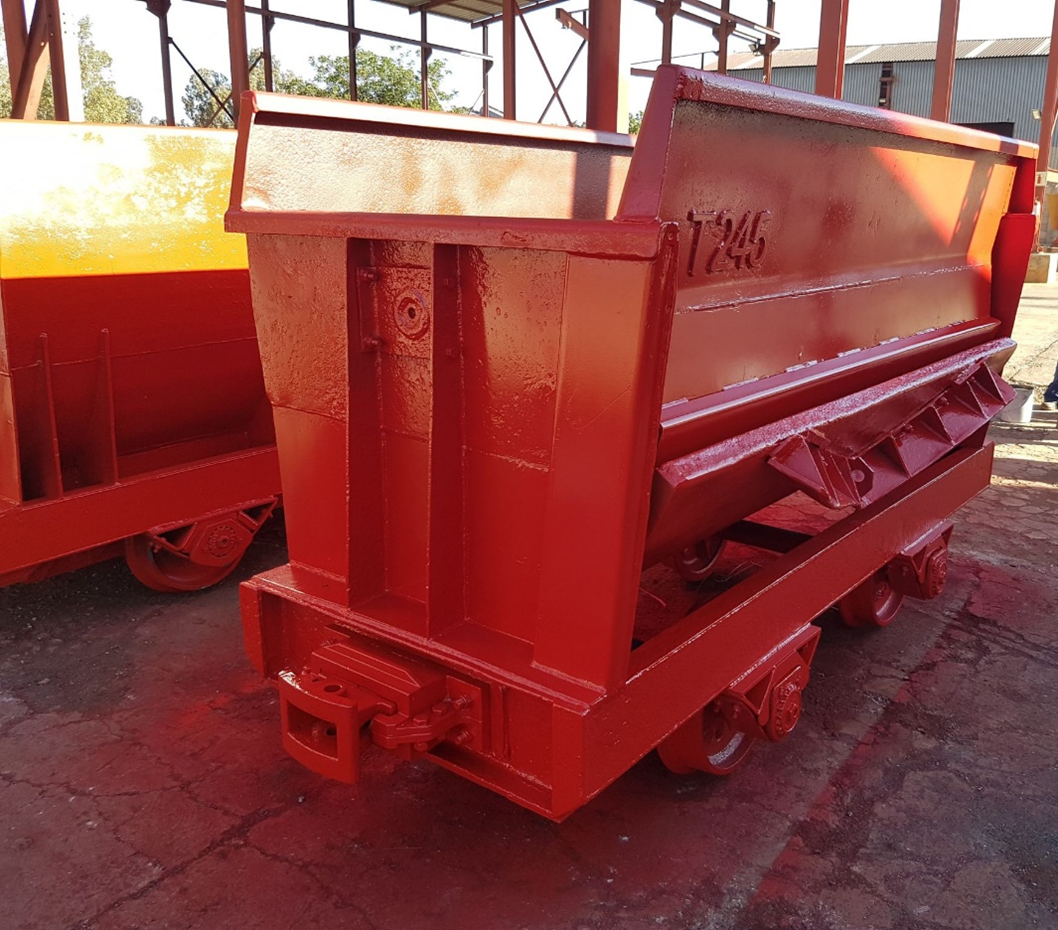
\includegraphics[width=0.8\textwidth, height=0.8\textheight, keepaspectratio]{img/Hopper.png}}
    \caption{Photo of hopper}
\end{figure}
\begin{figure}[H]
    \centering
    \makebox[\textwidth][c]{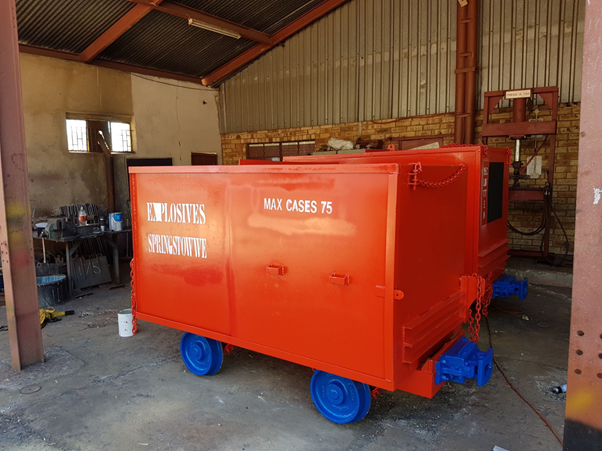
\includegraphics[width=0.8\textwidth, height=0.8\textheight, keepaspectratio]{img/ExplosiveCar.png}}
    \caption{Photo of explosive car}
\end{figure}
\section{Discuss the decision variables for the problem.}
\textbf{There are two decision variables:}
\begin{enumerate}
    \item X1: the number of hoppers to be produced.
    \item X2: The number of explosive cars to be produced.
\end{enumerate}
Both decision variables are made out of different inventory at Nuwelco: \\\\
\textbf{Needed for one hopper:}
\begin{enumerate}
    \item Welding Rods/Wire: 5 Roles of 20kg welding rod/wire rolls.
    \item Steel Plates: 10 sheets (3mm thickness).
    \item Cast-Iron Wheels: 4 Wheels.
    \item Dolly wheel: 1 Unit.
    \item Bolts: 100 Pieces.
    \item Nuts: 100 Pieces.
    \item Paint/Coating: 5 Drums containing 2 Liters of paint.
    \item Buffers: 4 Units.
    \item Wheel Rubbers: 8 pieces.
\end{enumerate}
\textbf{Needed for on explosive car:}
\begin{enumerate}
    \item Welding Rods/Wire: 10 Roles of 20kg welding rod/wire rolls.
    \item Steel Plates: 15 sheets (5mm thickness).
    \item Cast-Iron Wheels: 4 wheels.
    \item Rubber Lining: 2 Units of 3-meter lining.
    \item Bolts: 150 Pieces.
    \item Nuts: 150 Pieces.
    \item Paint/Coating: 10 Drums containing 2 Liters of paint.
    \item Buffers: 6 Units.
    \item Wheel Rubbers: 12 Pieces.
\end{enumerate}
By using the mixes above, a hopper or an explosive car can be produced (if available inventory allows for it). 
\section{Discuss the objective function for the problem.}
Pieter Swanepoel has outlined several key priorities for this period. His primary priority is to cap the workload at 180 hours to avoid overtime costs, which could diminish the project's profitability. His second priority is to achieve a minimum profit of R2,500,000 from the job. This sum will allow him to invest in a new CNC machine, complete construction on his second workshop, take a family vacation, and set aside funds for additional stock to fulfil future orders. His third priority is to further restrict working hours to 150 due to Eskom's monthly load shedding schedule, which limits their operational capacity without a generator.  His fourth and fifth priorities are to limit the usage of bolts (priority 4) and nuts (priority 5) to 3500 units each. This ensures sufficient inventory remains for the following month's requirements.

The objective function is as follow: P1d1+, P2d2-, P3d3+, P4d4+, P5d5+ \\\\
\textbf{The objective function means the following:}
\begin{enumerate}
    \item P1d1+: Minimize the chance of the deviational variable exceeding the base 180 hours. This is to ensure that no overtime money needs to be paid to the labour (first priority). 
    \item P2d2-: Minimize the chance of the deviational variable underachieving a profit of R2500000. This is to ensure that Pieter Swanepoel has the necessary funds for personal and business-related tasks (second priority). 
    \item P3d3+: Minimize the chance of the deviational variable exceeding the 150 hours because of load shedding (third priority).
    \item P4d4+: Minimize the chance of the deviational variable exceeding 3500 bolts (priority 4).
    \item P5d5+: Minimize the chance of the deviational variable exceeding 3500 nuts (priority 5).
\end{enumerate}
\section{Discuss the constraints, goal constraints, and the deviational variables.}
\textbf{All constraints found at question 5 answer and in order.}
\subsection{Goal constraints}
\begin{itemize}
    \item 1: Constraint that ensures no more than 180 hours of labour is done.
    \item 2: Constraint that wants 2500000 or more profit.
    \item 3: Constraint that ensures no more than 150 hours of labour is done because of load shedding.
    \item 4: Constraint limiting utilization of nuts to 3500 nuts.
    \item 5: Constraint limiting utilization of bolts to 3500 bolts.
\end{itemize}
\subsection{Normal constraints}
\begin{itemize}
    \item 6: Constraint limiting utilization of welding rots/wire to 250 units.
    \item 7: Constraint limiting steel plate 3mm utilization to 135 units.
    \item 8: Constraint limiting steel plate 5mm utilization to 300 units.
    \item 9: Constraint limiting cast iron wheel utilization to 125 units.
    \item 10: Constraint limiting dolly wheel utilization to 15 units.
    \item 11: Constraint limiting paint coating utilization to 250 units.
    \item 12: Constraint limiting buffers utilization to 200 units.
    \item 13: Constraint limiting wheel rubber utilization to 300 units.
    \item 14: Constraint limiting rubber lining utilization to 50 units.
    \item 15: Constraint limiting max hoppers to 10.
    \item 16: Constraint limiting max explosive carts to 15.
    \item 17: Non-negative constraint.
\end{itemize}
\subsection{Deviational variables}
\begin{itemize}
    \item d1: Aims to limit the labour hours to 150 hours (minimize overachieving).
    \item d2: Aims to make a minimum profit of 2500000 (minimize underachieving).
    \item d3: Aims to further limit the labour hours to 150 hours (minimize overachieving).
    \item d4: Aims to limit to use of bolts to 3500 (minimize overachieving).
    \item d5: Aims to limit to use of nuts to 3500 (minimize overachieving).

\end{itemize}
\newpage
\section{Provide the complete mathematical formulation of the model.}
\begin{figure}[H]
    \centering
    \makebox[\textwidth][c]{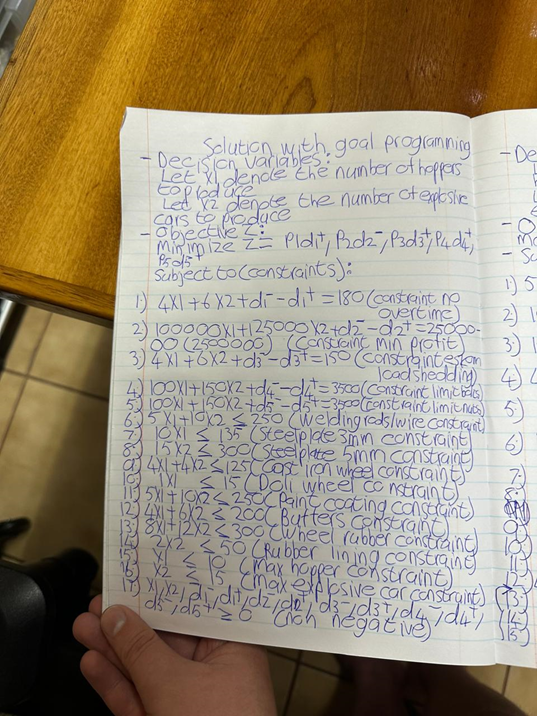
\includegraphics[width=1.1\textwidth, height=1.1\textheight, keepaspectratio]{img/Formulation paper.png}}
    \caption{Formulation on paper for the model.}
\end{figure}
\clearpage
\section{Briefly explain the solution process (i.e. software, order of steps) you followed. }
\begin{enumerate}
    \item Read the scenario to deeply understand the problem.
    Ignored the goal programming and wrote a normal linear programming model on paper.
    \item Solved the linear programming model in Excel using solver.
    \item Formulated the goal programming model on Excel.
    \item Solved the goal programming model in Excel using solver and in Python using pulp.
    \item Analysed the results from the solver/pulp.
    \item Wrote a conclusion about the results found.
\end{enumerate}
\section{Provide the solution.}
X1 = 10, X2 = 15, d1- = 50, d2+ = 375000, d3- = 20, d4- = 250, d5- = 250
\section{Discuss the meaning of the solution (50-100 words).}
Nuwelco was able to complete the order from CS\&IS mines with extra resources. Even when implementing the goal constraints, there was still additional resources left. Therefore, the order was completed (X1 = 10 and X2 = 15) within a months’ time and there were extra resources left including: d1- = 50 (extra hours of Labour), d2+ = 375000 (Extra capital left), d3- = 20 (Extra labour hours left), d4- = 250 (Extra bolts left), d5- = 250 (Extra nuts left).
\newpage
\section{Excel solutions}
\begin{figure}[H]
    \centering
    \makebox[\textwidth][c]{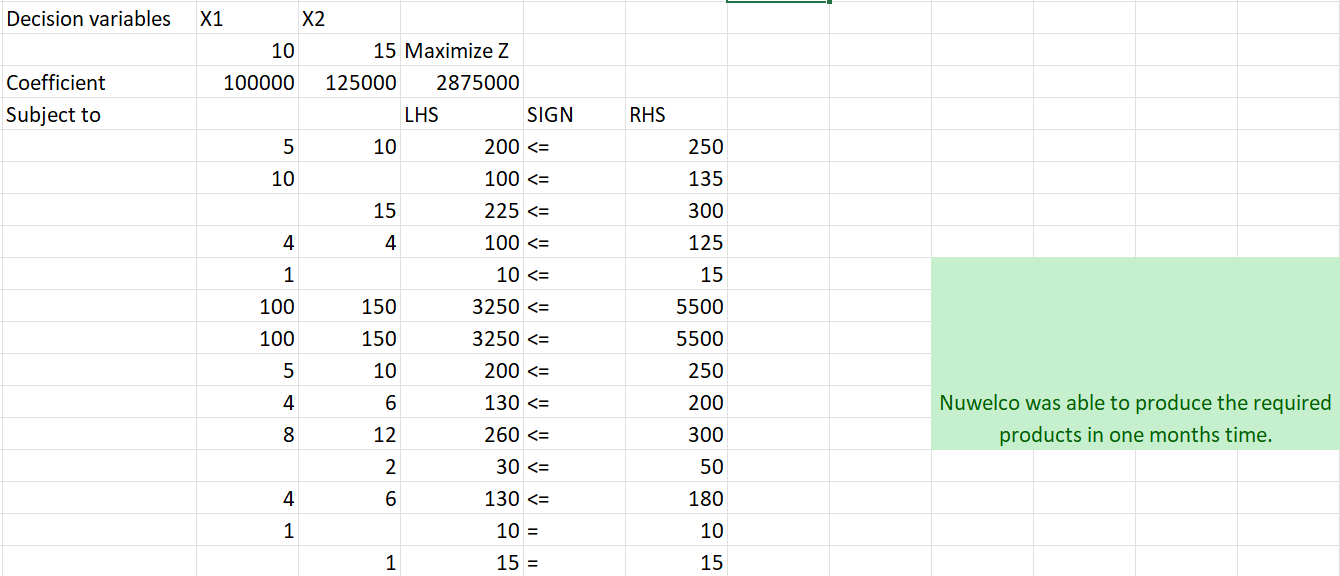
\includegraphics[width=1.3\textwidth, height=1.3\textheight, keepaspectratio]{img/SolutionExcel.png}}
    \caption{Excel solution for normal linear programming model.}
\end{figure}
\begin{figure}[H]
    \centering
    \makebox[\textwidth][c]{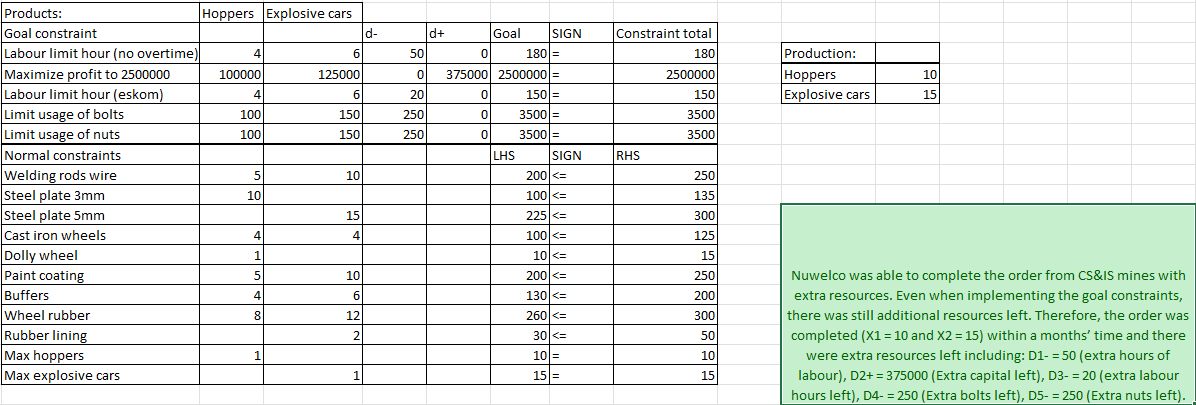
\includegraphics[width=1.3\textwidth, height=1.3\textheight, keepaspectratio]{img/SolutionExcelGoal.png}}
    \caption{Excel solution for goal programming model.}
\end{figure}
\section{Python solution (Linear programming)}
\begin{figure}[H]
    \centering
    \makebox[\textwidth][c]{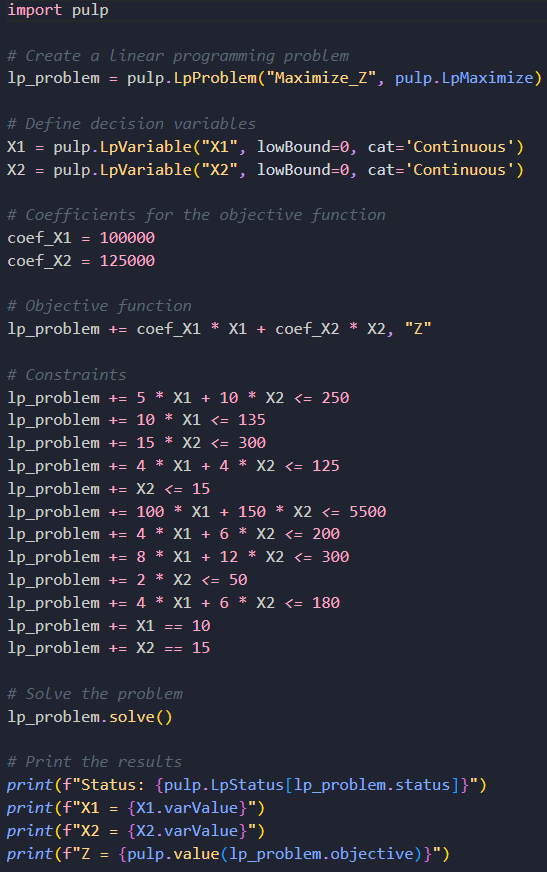
\includegraphics[width=0.7\textwidth, height=0.7\textheight, keepaspectratio]{img/PythonSolution.png}}
    \caption{Code for python linear programming solution.}
\end{figure}
\begin{figure}[H]
    \centering
    \makebox[\textwidth][c]{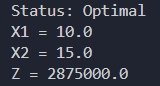
\includegraphics[width=0.4\textwidth, height=0.4\textheight, keepaspectratio]{img/PythonSolutionResult.png}}
    \caption{Results for python linear programming solution.}
\end{figure}
\section{Python solution (Goal programming)}
\begin{figure}[H]
    \centering
    \makebox[\textwidth][c]{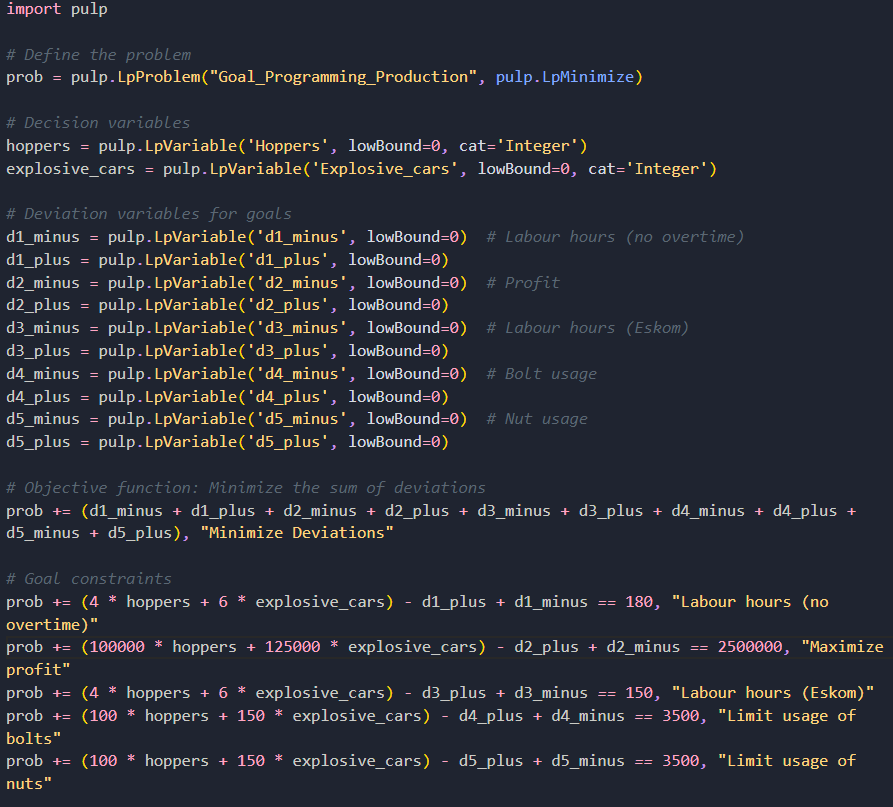
\includegraphics[width=1.3\textwidth, height=1.3\textheight, keepaspectratio]{img/PythonSolutionGoal1.png}}
    \caption{Code for python goal programming solution 1.}
\end{figure}
\begin{figure}[H]
    \centering
    \makebox[\textwidth][c]{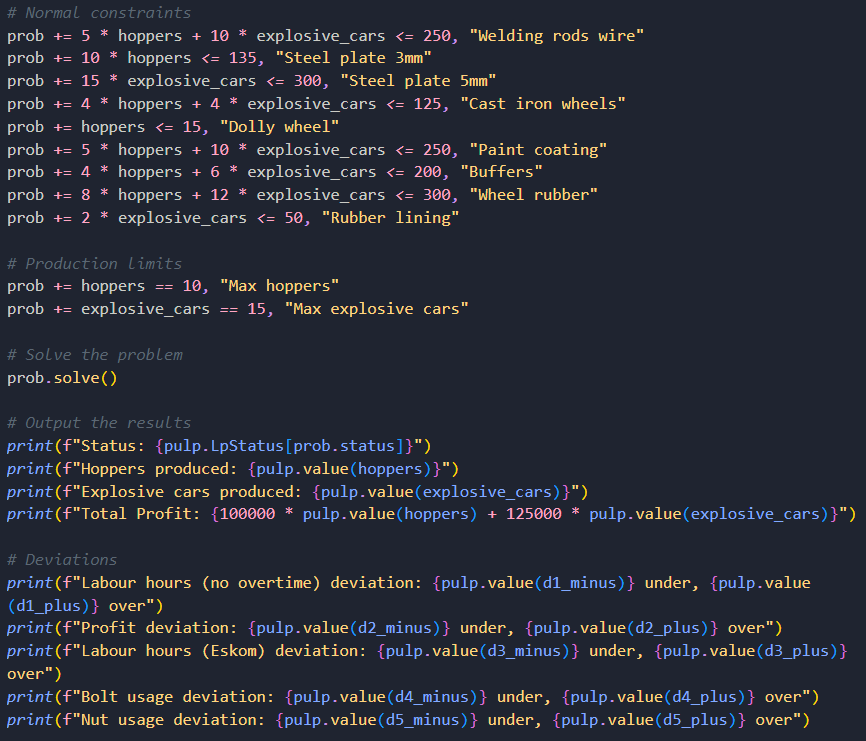
\includegraphics[width=1.3\textwidth, height=1.3\textheight, keepaspectratio]{img/PythonSolutionGoal2.png}}
    \caption{Code for python goal programming solution 2.}
\end{figure}
\begin{figure}[H]
    \centering
    \makebox[\textwidth][c]{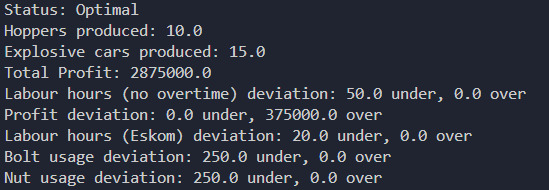
\includegraphics[width=0.7\textwidth, height=0.7\textheight, keepaspectratio]{img/PythonSolutionResultGoal.png}}
    \caption{Results for python goal programming solution.}
\end{figure}
\end{document}
